\section{Data Analysis: Community}

\subsection{Where Did Participants Come From?}

\begin{figure}
  \centering
  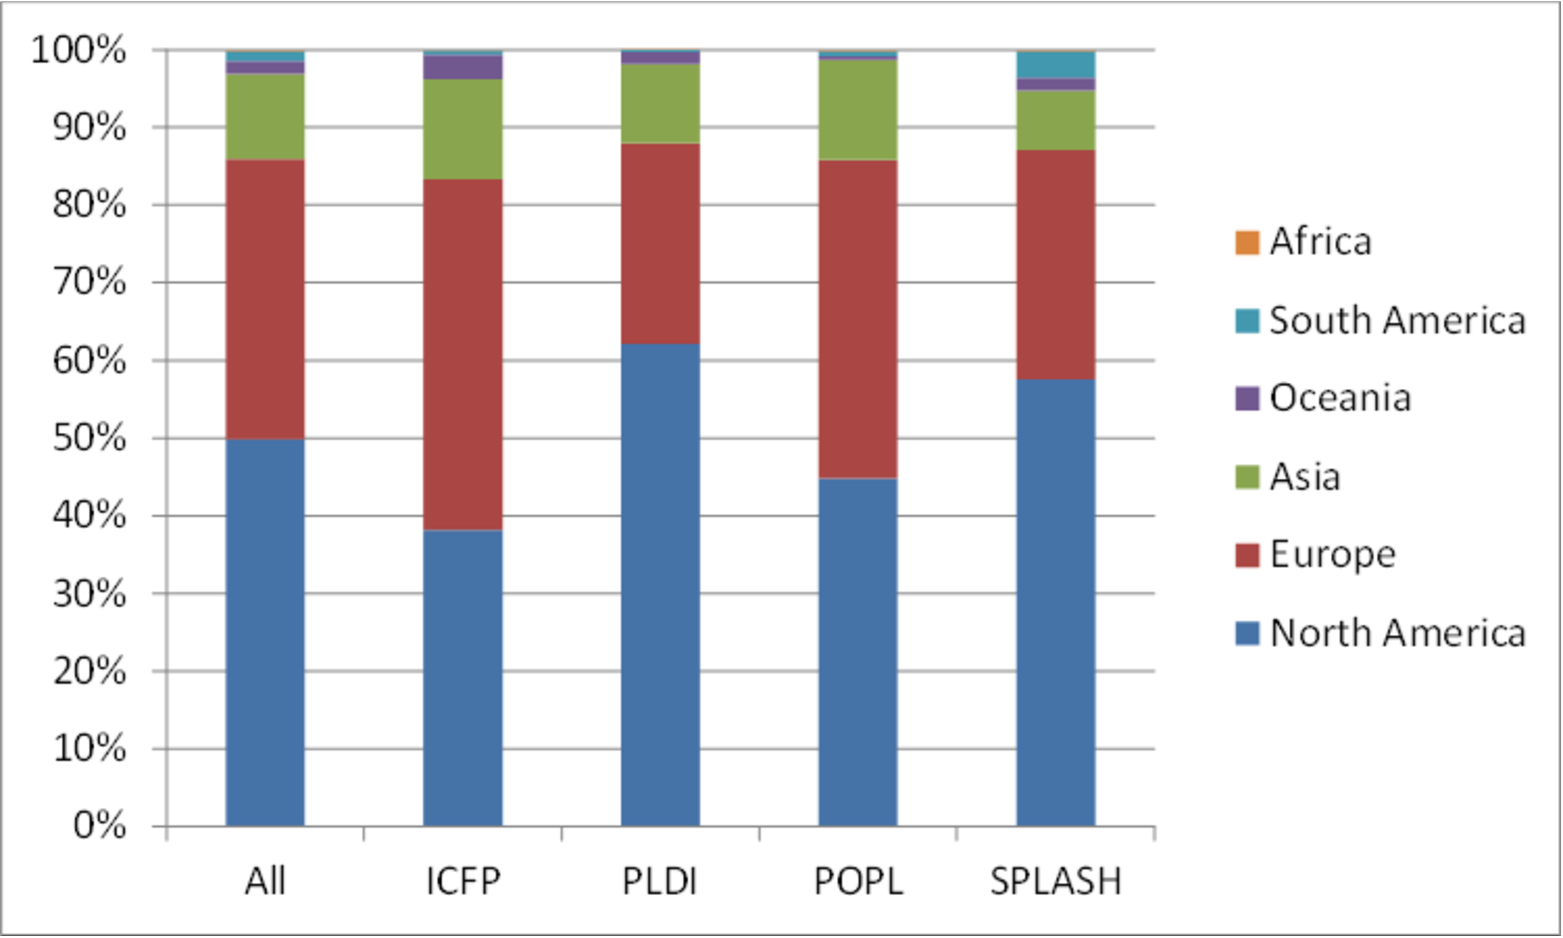
\includegraphics[width=0.7\textwidth]{figs/ParticipantsOrigin.pdf}
  \caption{Overall origin of participants.}
  \label{fig:continents}
\end{figure}

Figure~\ref{fig:continents} shows where all participants came from. Taken as a whole, these conferences attracted 50\% participants from North America, 36\% from Europe, 11\% from Asia, 2\% from Oceania, 1\% from South America, and less than 0.2\% from Africa. The chart also shows that, during this period, ICFP and POPL attracted a more balanced ratio of North Americans and Europeans than PLDI and SPLASH, the latter two dominated by North Americans. This overall picture, however, hides some interesting facts pertaining to the relation between the conferences' locations and the origin of the participants. 

Figure~\ref{fig:continents_per_conference} shows a more detailed break down of the origin of participants for each conference, showing also the geographic region where the conferences were held. These charts make it clear that the location of the conferences had a substantial effect on attracting people from the same geographic areas. That effect is quite visible for ICFP and POPL, with noticeable ups and downs of the colored bars between North American and European participants when the conferences were located in North America and Europe, respectively. The same is true for when the conferences were located in Asia, as those attracted a much higher number of Asian participants. ICFP11, ICFP16, and POPL15 are good examples of conferences that have achieved a good balance between North American, European, and Asian participants; they were all held in Asia. The effect is also visible for SPLASH, which has always been held in North America, except in 2016, when it was held in Europe, with a visible influx of European participants. 

\begin{figure}
  \centering
  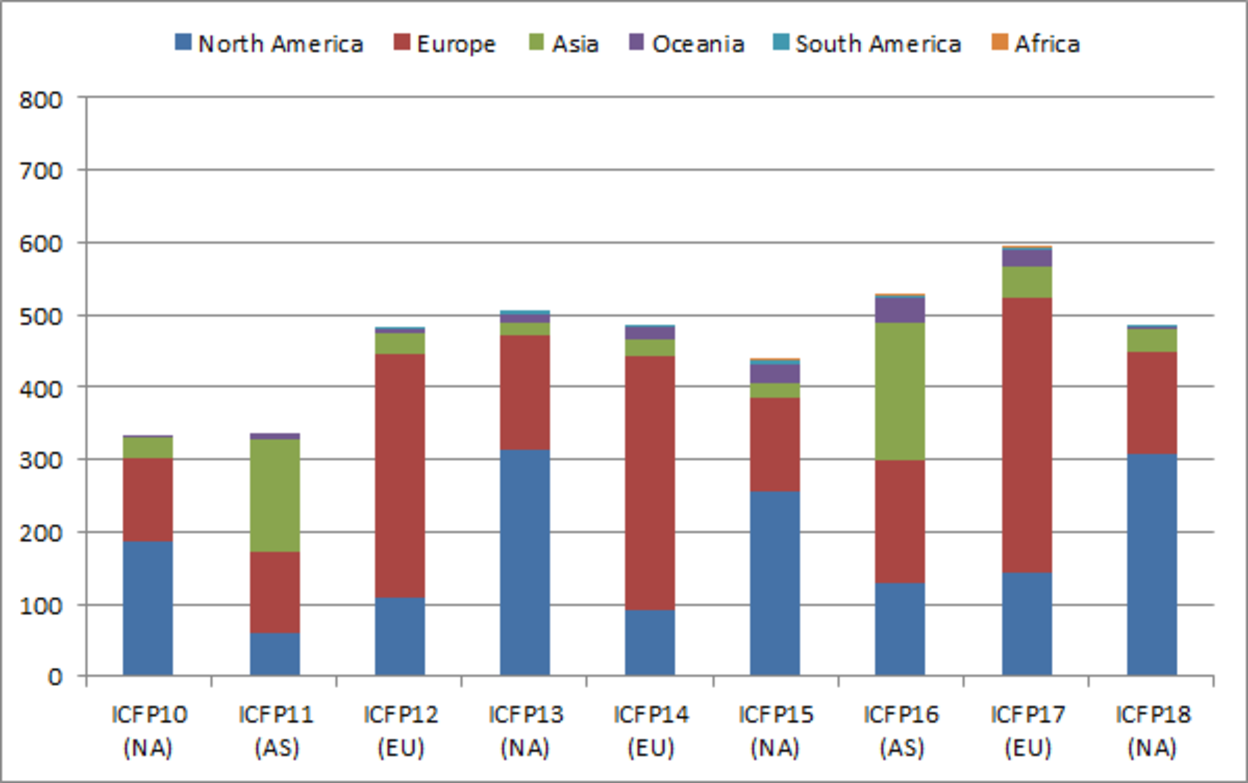
\includegraphics[width=0.45\textwidth,height=1.8in]{figs/ParticipantsOriginICFP.pdf}
  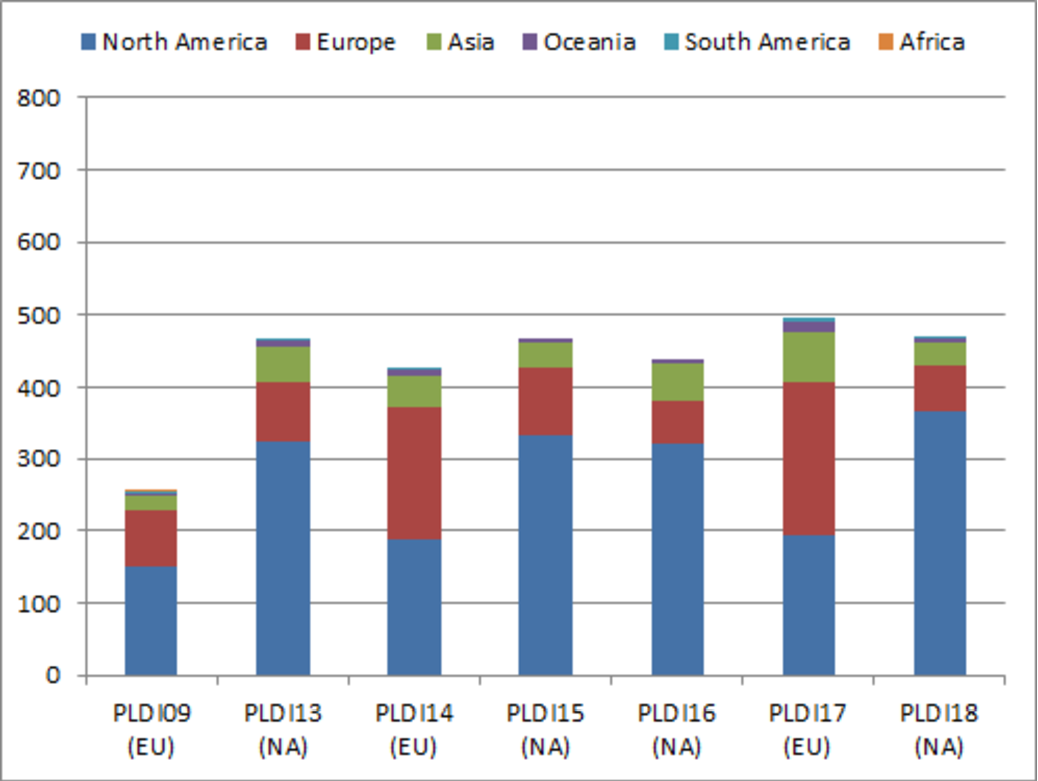
\includegraphics[width=0.45\textwidth,height=1.8in]{figs/ParticipantsOriginPLDI.pdf}
  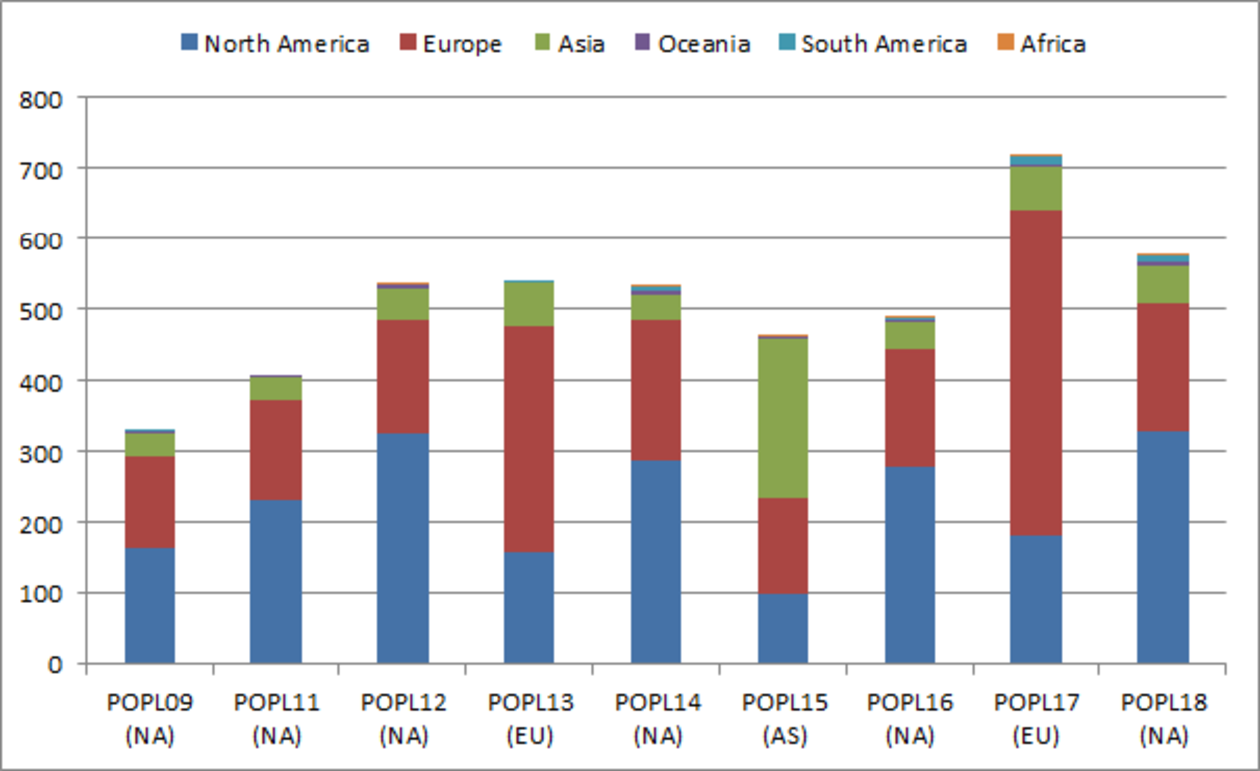
\includegraphics[width=0.45\textwidth,height=1.8in]{figs/ParticipantsOriginPOPL.pdf}
  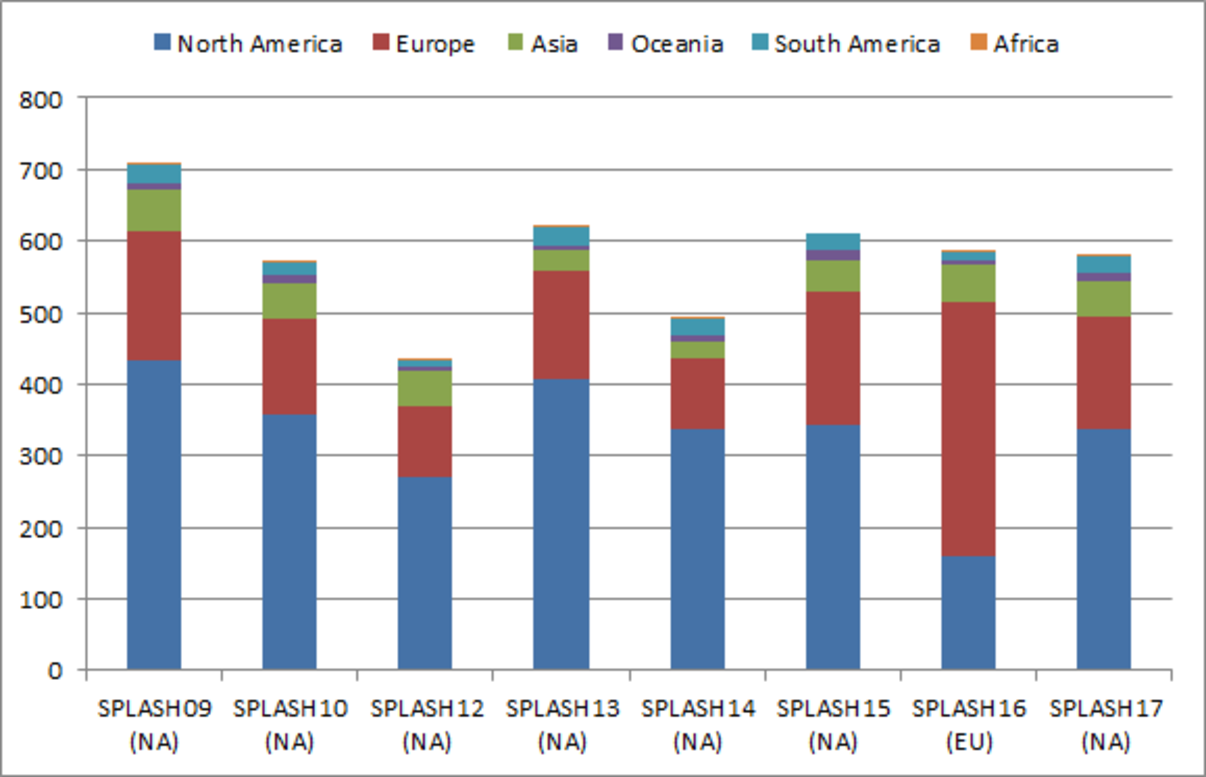
\includegraphics[width=0.45\textwidth,height=1.8in]{figs/ParticipantsOriginSPLASH.pdf}
  \caption{Origin of participants for each conference.}
  \label{fig:continents_per_conference}
\end{figure}


This data shows that the goal of geographic inclusion was, indeed, accomplished by organizing the conferences in diverse geographic areas of the world. It also places Figure~\ref{fig:continents} into a broader context: a naive interpretation of that chart might lead us to conclude that North America and Europe are where most of this community is, but it is not that simple. Because of the regional effect on participation, the distribution of participants also reflects the fact that most of these conferences were held in North America and Europe (30), only a few were held in Asia (3), and none was held in South America, Oceania, or Africa.


\subsection{How Often Did Participants Attend These Conferences?}


\begin{figure}
  \centering
  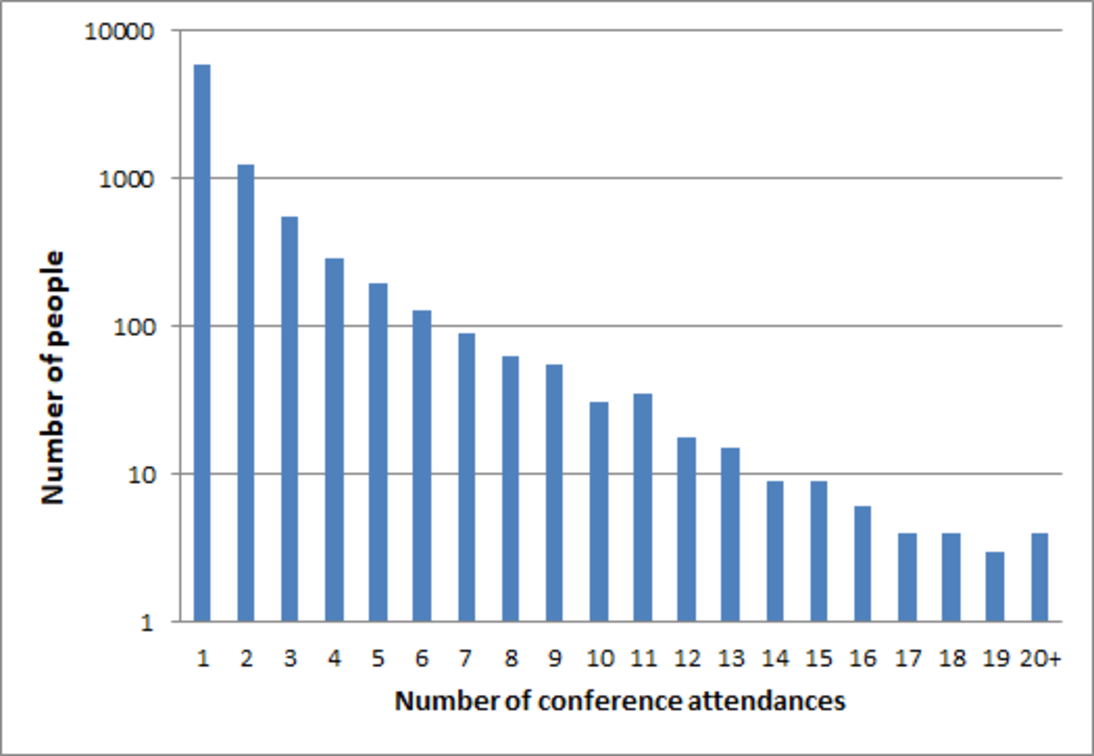
\includegraphics[width=0.6\textwidth]{figs/AttendanceHist.pdf}
  \caption{Histogram of attendance.}
  \label{fig:hist_attendance}
\end{figure}

Figure~\ref{fig:hist_attendance} shows how often the same participants attended multiple conferences. At the extremes, 6,009 people (69\%) attended only 1 conference, and 4 people attended 20 or more conferences. Participation is dominated by single-conference participants, which reflects the large and transient student population. The pattern is similar for each conference series, shown in Figure~\ref{fig:hist_attendance_per_conference}.

\begin{figure}
  \centering
  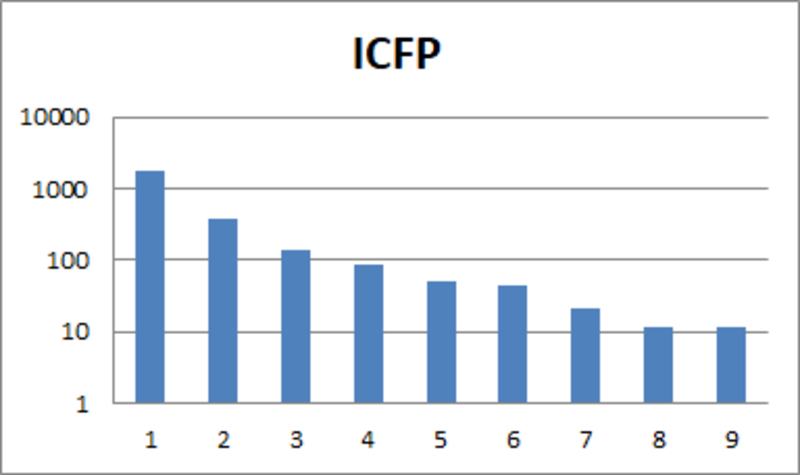
\includegraphics[width=0.45\textwidth,height=1.5in]{figs/AttendanceHistICFP.pdf}
  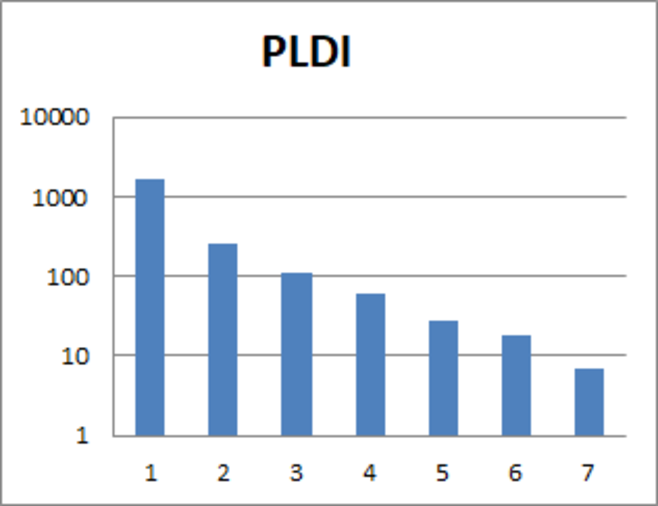
\includegraphics[width=0.4\textwidth,height=1.5in]{figs/AttendanceHistPLDI.pdf}
  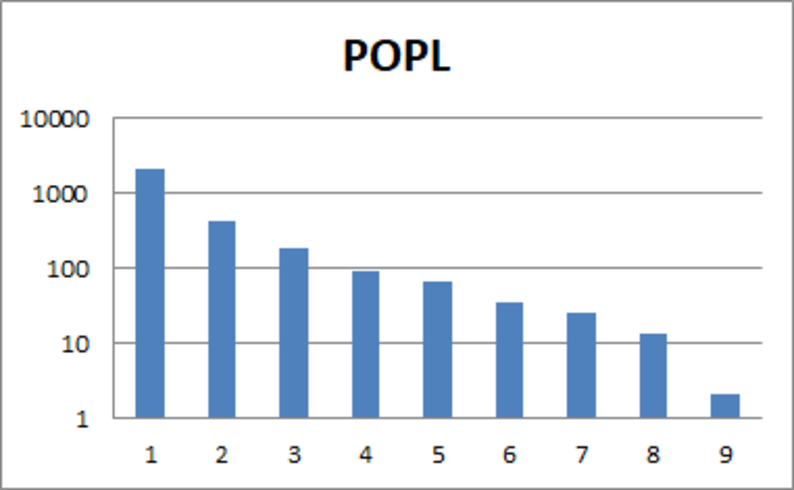
\includegraphics[width=0.45\textwidth,height=1.5in]{figs/AttendanceHistPOPL.pdf}
  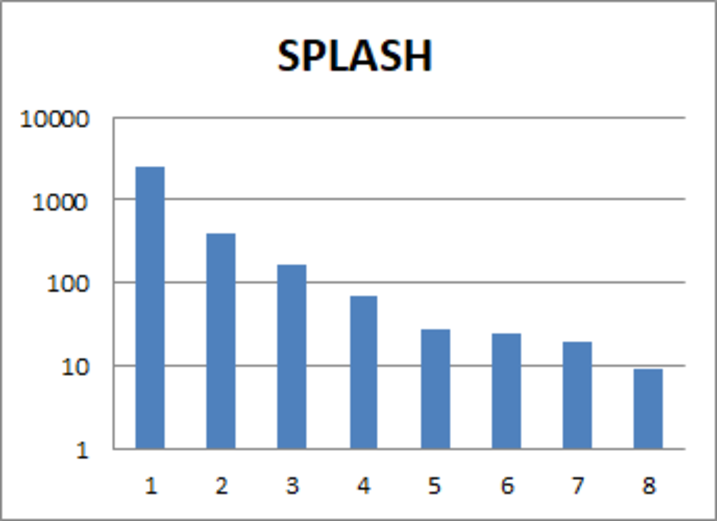
\includegraphics[width=0.4\textwidth,height=1.5in]{figs/AttendanceHistSPLASH.pdf}
  \caption{Histogram of attendance for each conference series.}
  \label{fig:hist_attendance_per_conference}
\end{figure}


\subsection{What Was the Participation Overlap Between These Conferences?}

Figure~\ref{fig:overlap} shows the overlap in participants between the various conferences. The overlap reflects the permanence vs. transience of the participants over time in SIGPLAN conferences. In principle, it is desirable to have a balance between repeat participants and newcomers. Communities that don't attract new participants tend to stagnate; but communities that don't have a core of repeat participants tend to lose focus.

Not surprisingly, the strongest overlaps are within each conference series over the years; this shows that there is, indeed, a certain community associated with each conference series that tends to repeat participation. The highest overlap of all was between ICFP'16 and ICFP'17, with 180 repeaters. The four conference series show a healthy balance between repeat participation and newcomers. 

There is also some, although weaker, overlap between conferences in different series. For example, there is a somewhat surprising overlap between PLDI and POPL, followed by ICFP and POPL and by PLDI and SPLASH. The weakest overlaps are between ICFP and SPLASH, followed by ICFP and PLDI, and by POPL and SPLASH. It is unclear whether the overlap, or lack thereof, between these conference series is due to intellectual reasons or due to their dates. PLDI and POPL is the pair that is most distant in time, typically June and January, respectively. ICFP and SPLASH is the pair that is the closest in time, typically September and October. Time proximity may detract cross-participation.

\begin{figure}
  \centering
  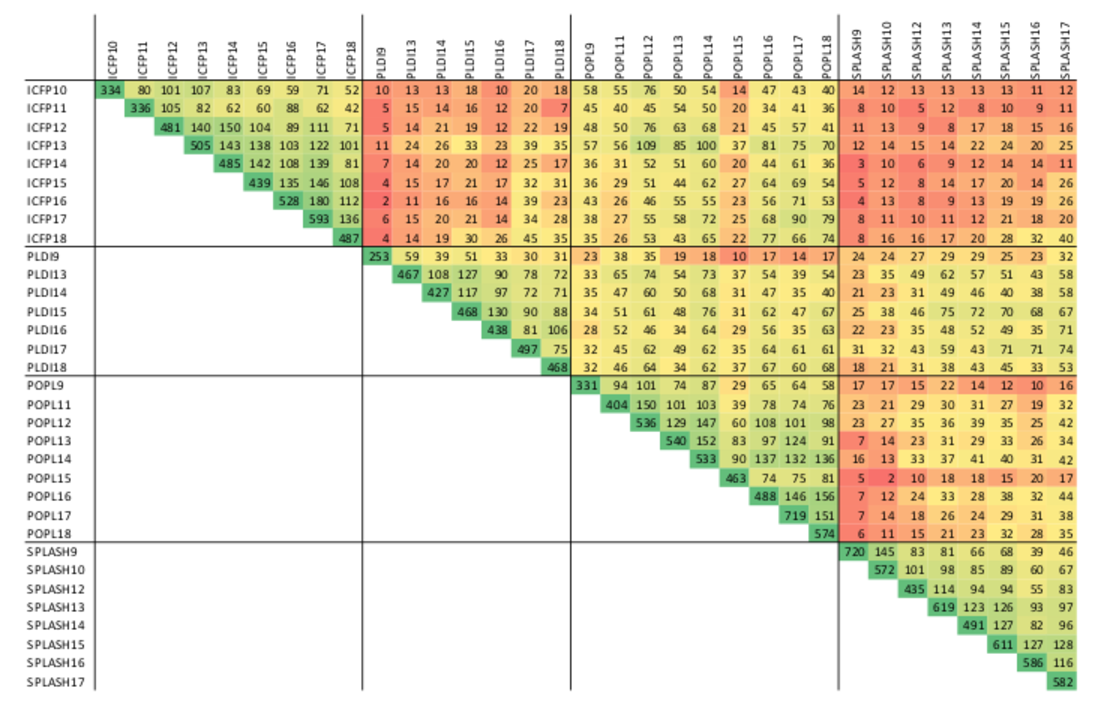
\includegraphics[width=\textwidth]{figs/OverlapAnalysis-crop.pdf}
  \caption{Conference participation overlap.}
  \label{fig:overlap}
\end{figure}
